% Paper I: mechanism + reheating closure + official low-ell likelihood.
% Springer SVJour3 class (the basis of the EPJC macro package).
\documentclass[twocolumn]{svjour3}

\usepackage{amsmath,amssymb}
\usepackage{graphicx}
\usepackage{booktabs}
\usepackage[hidelinks]{hyperref}

\newcommand{\Mpl}{M_{\rm Pl}}
\newcommand{\Mpc}{\,{\rm Mpc}^{-1}}

\journalname{Eur. Phys. J. C}

\begin{document}

\title{A nonsingular metric $f(R)$ completion of Starobinsky inflation
with a reheating-determined low-multipole feature}
\titlerunning{A nonsingular $f(R)$ completion of Starobinsky inflation}
\author{Stilian Pandev}
\authorrunning{S. Pandev}
\institute{Independent researcher \\ \email{stilianpandev@gmail.com}}
\date{Received: date / Accepted: date}

\maketitle

\begin{abstract}
We construct a metric $f(R)$ extension of Starobinsky inflation in which two
additional curvature operators, $R^{\,p+1}$ and $R^{\,2p+1}$ with integer
$p$, admit an exact constant-curvature solution with a single unstable
scalaron mode, allowing inflation to begin at a regular Euclidean
four-sphere rather than at a singularity. The construction is fixed by a
zero-work condition on the trace-flow wall in a declared integration
measure, and by a unit spectral gap on the
four-sphere, $\mu^2=d-1$; integrality of $p$ follows from analyticity of the
action at $R=0$. Two representative walls---the legacy coordinate rule and
the canonical invariant-measure choice---paired with minimal and conformal
Higgs couplings respectively, define the two model branches analyzed. The model retains the Starobinsky predictions
$n_s\simeq0.962$--$0.964$ and $r\simeq0.004$, and adds an approximately
$50\%$ localized deficit in the scalar power spectrum near
$k\sim10^{-4}\,\mathrm{Mpc}^{-1}$, with no tensor counterpart. The deficit
location is exactly degenerate between $p$ and the reheating history, but
the latter is calculable here because the low-curvature limit is exactly
$R+R^2/6M^2$: the coupled scalaron--radiation system yields
$N_*=50.6$--$51.6$, set by the Higgs curvature coupling, with an uncertainty
of $0.2$ e-folds against an integer spacing of $0.94$--$0.99$, so that
the degeneracy is closed and each integer predicts a definite feature location.
Propagating the exact spectra through CAMB, validated against CLASS to
$6\times10^{-4}$, and evaluating the official Planck 2018 low-$\ell$
Commander and SimAll likelihoods, we find that one integer of each branch is
excluded ($\Delta\chi^2=+13.4$ and $+8.5$), that the preferred integers give
$\Delta\chi^2_{TT+EE}=-1.5$ to $-1.7$, and that the evidence marginalized
over the integer ladder is $+1.0$, consistent with a statistical
fluctuation; the deficit itself lies below cosmic variance and cannot be
confirmed by the low-$\ell$ CMB. All numerical results are reproducible from
the released code.
\keywords{Inflation \and $f(R)$ gravity \and Primordial power spectrum
\and Cosmic microwave background \and Reheating}
\end{abstract}

\section{Introduction}
\label{sec:intro}
Starobinsky's $R^2$ inflation \cite{Starobinsky1980} remains the observational
benchmark of the inflationary paradigm: with a single mass scale fixed by the
scalar amplitude it predicts $n_s\simeq0.963$ and $r\simeq0.004$, comfortably
inside the Planck constraints \cite{Planck2018X}. In its original form the
model was, moreover, born nonsingular: it began in an unstable de Sitter
state supported by the conformal anomaly, whose decay launched the
scalaron-driven quasi-de Sitter expansion \cite{Starobinsky1980}; the
perturbation spectrum evolving from that nonsingular initial stage was
computed shortly afterwards \cite{Starobinsky1983}, and the quantum creation
of the universe into the unstable de Sitter phase was analyzed by Vilenkin
through a compact Euclidean instanton \cite{Vilenkin1985}. A modern
realization of the same arc, from anomaly-induced de Sitter through a
graceful exit into the $R+R^2$ attractor, is given in \cite{Netto2016}. In
the version of the model used throughout modern cosmology, however, the
anomaly-supported stage is discarded: the truncation $R+R^2/6M^2$ extends
backward into a curvature regime where it has no particular authority, and
the classical history terminates in the usual singularity. Nonsingular
completions---the no-boundary proposal \cite{Lehners2023}, bouncing and
emergent scenarios---are then supplied from ingredients outside the
gravitational action.

This paper realizes the original scenario within a local, polynomial, metric
$f(R)$ theory. Two additional curvature operators create an exact
constant-curvature solution---a ``frozen horizon''---at $R_H=qM^2$: the
$f(R)$ counterpart of a Hawking--Moss saddle \cite{HawkingMoss1982}, with
precisely one unstable scalaron direction whose growth takes the universe
out of the horizon, through a brief fast-roll phase, and onto the ordinary
Starobinsky attractor. Where the anomaly-supported de Sitter state has its
curvature and decay rate fixed as outputs of the anomaly coefficients, here
both are independent algebraic data of the action, set by the conditions of
Sec.~\ref{sec:construction}; the de Sitter root is exact rather than
one-loop-induced; and the family of such completions is discrete. The
Euclidean continuation of the horizon is a regular four-sphere, so the
classical singularity is replaced by a compact saddle; the quantum-state
analysis of that saddle (integration contour, classicalizing thimble, and the
discrete mode-crossing kernel near the waist) is developed in a companion
paper \cite{PandevII} and is not needed for the phenomenology discussed here.

A localized suppression of scalar power from a fast-roll stage preceding
slow roll is itself a well-studied mechanism: it arises generically in exits
from unstable de Sitter states \cite{Linde2001}, from pre-inflationary
kinetic domination \cite{Contaldi2003,Boyanovsky2006}, from discontinuities
in the inflaton potential \cite{Starobinsky1992}, and in punctuated
\cite{Jain2009} and whipped \cite{Hazra2014,Hazra2016} inflation;
suppressed-power primordial spectra have been reconstructed directly from
the Planck data \cite{Planck2018X}, and infrared-cutoff families continue to
be confronted with current data \cite{Upadhyay2026}. The present
construction belongs to this family at the
level of the mechanism---the fast-roll shoulder of
Sec.~\ref{sec:construction} plays the role of the pre-slow-roll stage---and
differs from it in three respects. The fast-roll phase is not an initial
condition but an exact solution of the gravitational action itself; the
scale of the feature is not scanned or fitted but computed, through the
reheating closure of Sec.~\ref{sec:reheating}; and the model space is
discrete, an integer ladder rather than a continuous parameter, which is
what allows individual members to be excluded outright rather than merely
constrained.

Beyond the construction itself, the analysis makes a methodological point
that applies to primordial feature models generally: a model that does not
compute its reheating history does not predict the location of its feature.
The wall imprints a
localized scalar power deficit a fixed number of e-folds before the end of
inflation, but converting that into a wavenumber requires the pivot's e-fold
distance $N_*$, and we show that the integer label $p$ of the model family is
exactly degenerate with $N_*$ (Sec.~\ref{sec:reheating}). This degeneracy is closed by the structure of the model itself: its
low-curvature limit is exactly Starobinsky, so that reheating is calculable
rather than parameterized, and the chain
$A_s\to M\to\Gamma_\phi\to T_{\rm re}\to N_*$ closes with an uncertainty of
$\sigma(N_*)\simeq0.2$ e-folds against an integer spacing of $0.94$--$0.99$
e-folds,
so that adjacent integers predict cleanly separated feature locations and
the location becomes a genuine prediction of each completion.

The observational reach of the model is bounded, and is quantified as
follows. The predicted deficit lies at the lowest multipoles, where
cosmic variance is of order $50\%$ per mode; even a full-sky, noiseless
experiment could not establish it beyond approximately $2\sigma$, and no
detection claim is made. The data can, however, exclude: evaluating the
official Planck 2018 low-$\ell$ likelihoods on the exact spectra rejects one
integer of each model branch ($\Delta\chi^2=+13.4$ and $+8.5$), while the
surviving integers improve the fit by $-1.5$ to $-1.7$, with a marginalized
value of $+1.0$ that is consistent with noise. The delineation of this
boundary, together with the closed scale chain and the reproducibility of
every numerical result from the released code, constitute the principal results reported
here.

Section~\ref{sec:construction} defines the construction and the two
conditions imposed on its gravitational sector.
Section~\ref{sec:stability} establishes stability and the background
solution. Section~\ref{sec:reheating} presents the degeneracy and its
reheating closure. Section~\ref{sec:spectra} computes the primordial spectra
and shows which of their properties are and are not observable.
Section~\ref{sec:cmb} propagates them to the CMB and evaluates the official
likelihoods. Section~\ref{sec:discussion} collects the assumption ledger,
falsification criteria, the horizon-thermodynamic properties of the
solution, and the ultraviolet program;
Section~\ref{sec:conclusions} summarizes the results.

\section{The frozen-horizon construction}
\label{sec:construction}
This section defines the action, establishes the exact de Sitter root and the
two conditions that fix it, and shows that the resulting model family is
discrete.

\subsection{Action and trace-flow wall}
The inflationary sector is metric $f(R)$ gravity,
$S=\tfrac12\Mpl^2\int d^4x\sqrt{-g}\,f(R)$, with $f(R)=M^2 g(x)$ and
$x=R/M^2$. Writing $y=x/q$, $z=y^p$ for an integer $p$ and horizon curvature
$q$, the curvature function is
\begin{equation}
g(x)=x+\frac{x^2}{6}
-\frac{(\alpha-1)\,q}{p-1}\,y^{\,p+1}
+\frac{\alpha\,q}{2p-1}\,y^{\,2p+1},
\label{eq:g}
\end{equation}
whose low-curvature limit is exactly the Starobinsky action
$R+R^2/6M^2$. The two high powers deform the theory only near $x=q$. The
construction is organized around the normalized trace-flow slope
$S\equiv(2g-xg')/x$, for which Eq.~(\ref{eq:g}) gives the exact identity
\begin{equation}
S(z)=(1-z)(1+\alpha z),
\label{eq:wall}
\end{equation}
for every $x$ and every $p$: the $R^2/6$ term cancels identically from $S$,
which is why the Starobinsky limit coexists with the wall. $S$ has a direct
reading as the Einstein--Hilbert fraction of the action: $S=1$ for pure $R$,
$S=0$ for pure $R^2$. The point $S=0$ is where the theory becomes locally
scale invariant, and since a constant-curvature solution satisfies
$Rf_R-2f=0$ \cite{BarrowOttewill1983}, i.e.\ $S=0$, the wall's zero at $z=1$
furnishes the exact de Sitter root
\begin{equation}
R_H=qM^2 .
\end{equation}
We refer to this solution as the frozen horizon: an exact, nonsingular de
Sitter state arising within the $f(R)$ sector itself, from which inflation
begins. De Sitter points of polynomial $f(R)$ Lagrangians of precisely this
class, $R+R^2+R^n$, have been catalogued and their stability classified
\cite{Pham2024,Huang2013,Artymowski2015}; what distinguishes the present
construction is not the existence of the root but the two conditions imposed
on it below, which fix the shape of the wall and the spectrum of the
instability rather than merely its sign.

\subsection{The zero-work condition and its measure}
\label{sec:measure}
The boundary conditions $S(0)=1$ and $S(1)=0$ leave the quadratic wall a
one-parameter family, Eq.~(\ref{eq:wall}). The remaining coefficient is fixed
by a zero-work condition, $\int_{0}^{1}(S-1)\,d\mu=0$, taken over the full
wall from $R=0$ to the horizon ($z=0$ to $1$). The condition acquires content only once
the measure $d\mu$ is declared, and coordinate invariance narrows
but does not eliminate this freedom:
\begin{center}
\small
\setlength{\tabcolsep}{4pt}
\begin{tabular}{lcc}
\hline
measure & $\alpha$ & $S_{\max}$ \\
\hline
$dz$ (wall coord.; not inv.) & $3$ & $4/3$ \\
$d\ln R$ & $2$ & $1.125$ \\
$dR$ & $2+1/p$ & $1.128$ \\
$d\phi\propto d\ln f_R$ (canonical) & $2.8088$--$2.8096$ & $1.291$ \\
\hline
\end{tabular}
\end{center}
The first three entries are exact. With $S-1=(\alpha-1)z-\alpha z^2$ and
$x=qz^{1/p}$ the condition integrates in elementary form in each case: $dz$
gives $\tfrac12(\alpha-1)=\tfrac13\alpha$, hence $\alpha=3$; $d\ln R$ carries
the weight $dz/pz$ and gives $(\alpha-1)=\tfrac12\alpha$, hence $\alpha=2$
for every $p$; and $dR$ carries $z^{1/p-1}$ and gives
$(\alpha-1)p/(1+p)=\alpha p/(1+2p)$, hence $\alpha=2+1/p$, which is
$2.015873$ at $p=63$ and $2.015152$ at $p=66$. The two curvature-based
invariant measures therefore coincide in the large-$p$ limit. The canonical
measure alone admits no closed form, because its weight
$d\ln f_R/dz=(g''/g')\,dx/dz$ is built from the very wall it fixes; there
$\alpha$ is a fixed point of the wall against its own field-space measure,
and the quoted range is its variation across the viable integers.
The wall coordinate $z=(x/q)^p$ embeds the integer $p$ in its own definition,
so the $dz$ rule cannot be fundamental. Among invariant choices we adopt the
canonical scalaron field-space measure $d\phi=\sqrt{3/2}\,\Mpl\,d\ln f_R$ as
the primary branch, with $d\ln R$ (the renormalization-group-natural choice,
$\alpha=2$) as the principal alternative; since $\alpha$ controls
$S_{\max}=(1+\alpha)^2/4\alpha$ and hence the depth of the primordial feature
(Fig.~\ref{fig:wall}), the choice is observationally meaningful in principle.
The phenomenological sections analyze two walls: the canonical-measure wall
as the primary branch, and the $\alpha=3$ coordinate-rule wall---retained
not as a candidate fundamental choice but as a robustness branch,
demonstrating that every qualitative conclusion below (the exclusion of the
infrared member, the noise-level preference for a narrow one) is insensitive
to the measure. The shallower $d\ln R$ wall is quantified in
Sec.~\ref{sec:spectra}. The two branches are paired with minimal
($\xi_H=0$) and conformal ($\xi_H=\tfrac16$) matter couplings respectively;
as Sec.~\ref{sec:reheating} shows, a change of $\xi_H$ acts on the integer
ladder as a relabeling, so mixed pairings duplicate rather than extend the
analyzed set.
\begin{figure}
\centering
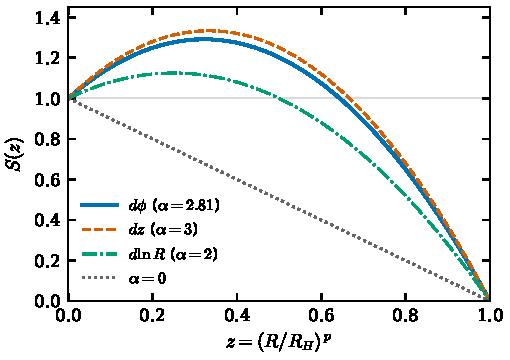
\includegraphics[width=\columnwidth]{figures/wall}
\caption{Trace-flow wall $S(z)=(1-z)(1+\alpha z)$ for the three integration
measures considered in Sec.~\ref{sec:measure} and, for contrast, the
shoulderless linear wall $\alpha=0$. The quantity $S$ is the
Einstein--Hilbert fraction of the action. The excursion above $S=1$ (the
fast-roll shoulder) generates the scalar power deficit; the linear wall
$\alpha=0$, which has no shoulder, produces no observable feature
(Sec.~\ref{sec:spectra}).}
\label{fig:wall}
\end{figure} The zero-work statement itself---that the integrated
trace deformation vanishes along the declared measure---is the single
arbitrary input of the gravitational sector, and Sec.~\ref{sec:discussion}
identifies its derivation (or refutation) from a fixed-function equation as
the decisive open problem.

\subsection{Unit spectral gap and the horizon curvature}
Scalar fluctuations on the Euclidean four-sphere of the horizon have
eigenvalues $\lambda_L=[L(L+3)-\mu^2]H_H^2$ with
$\mu^2=|m_H^2|/H_H^2$. Requiring exactly one negative mode---the
Coleman--De~Luccia condition for a legitimate exit direction
\cite{ColemanDeLuccia1980}---only bounds
$0<\mu^2<4$. The construction sharpens this to the unit-gap condition
$\lambda_1=H_H^2$, whose covariant content in $d$ dimensions is
\begin{equation}
\mu^2=d-1 ,
\end{equation}
i.e.\ $\mu^2=3$ here: the first stable harmonic sits exactly one Hubble unit
above zero. At a de Sitter point of an $f(R)$ theory in $d$ dimensions the
scalaron mass obeys $m^2/H^2=\tfrac{d(d-2)}{2}\,f_R/(Rf_{RR})-d$, so the
unit gap $\mu^2=d-1$ is equivalent to the local condition
$R f_{RR}=\tfrac{d(d-2)}{2}f_R$ at the horizon, and combined with
Eq.~(\ref{eq:wall}) it fixes the horizon curvature algebraically (at $d=4$):
\begin{align}
q&=p(1+\alpha)-3C(p,\alpha),\nonumber\\
C(p,\alpha)&=1-(\alpha-1)\frac{p+1}{p-1}+\alpha\frac{2p+1}{2p-1},
\end{align}
with the corollary $f_R(R_H)=p(1+\alpha)/3$. This sharpens the classical
de~Sitter stability criterion for fourth-order gravity \cite{MSS1988} from a
sign condition into an eigenvalue condition: the instability rate is fixed,
not merely required to exist. The unit gap
remains an axiom: it cannot be derived from the one-loop determinant of the
truncated theory in a regulator-independent way
(Appendix~\ref{app:unitgap}). The exit instability it produces has growth rate
$s=(\sqrt{21}-3)/2\simeq0.791$ and, at quadratic order, exactly one negative
direction on the half four-sphere. One consequence should be noted:
$\mu^2=3H_H^2$ exceeds the hilltop classicality bound $m^2<(3H/2)^2$ found
in scalar-field no-boundary analyses \cite{HHH2008}, so the emergence of
classical Lorentzian histories from this saddle is not automatic; it is
established by the classicalizing-thimble construction of the companion
paper \cite{PandevII}.

\subsection{Integrality of $p$}
The wall operators are $R^{\,p+1}$ and $R^{\,2p+1}$. If the low-curvature
action is a local analytic expansion about $R=0$---the ordinary
effective-field-theory requirement---then both exponents must be nonnegative
integers, hence
\begin{equation}
p\in\mathbb{Z},\qquad p>1 .
\end{equation}
The discreteness of the model family is therefore derived rather than
postulated; which integer is realized remains empirical. Beyond the observed
scalar amplitude, the construction thus has exactly two free inputs: the
integer $p$ and the zero-work measure of Sec.~\ref{sec:measure}. All
subsequent quantities---the horizon curvature, the exit rate, the spectral
feature, and the reheating history---are computed rather than fitted.

\section{Stability and background evolution}
\label{sec:stability}
Metric $f(R)$ gravity is equivalent to Einstein gravity plus a canonical
scalaron whenever $f_R>0$ and $f_{RR}>0$. Both hold everywhere on the
numerically integrated trajectory from the horizon to the end of inflation:
$\min f_R=1.6518$, attained at the exact end point $\epsilon=1$
($x\simeq1.955$), and $\min M^2f_{RR}=0.2912$ mid-trajectory
(Table~\ref{tab:candidate}). A remark on conventions: the value
$g'(2\sqrt3)=2.1547$ that a slow-roll treatment would quote for $\min f_R$
belongs instead to the $\epsilon_V=1$ criterion, which is reached $0.28$
e-folds earlier. The two end-of-inflation conventions must not be mixed, and
all e-fold counts in this paper use the exact one. The negative scalaron
mass at the horizon, $m_H^2=-3H_H^2$, is
the intended exit instability, not a ghost: the kinetic sector remains
healthy throughout. The curvature-singularity problem that afflicts
infrared-modified $f(R)$ dark energy \cite{Frolov2008} does not arise here:
with the coefficient of $R^{\,2p+1}$ positive, $f_R\to\infty$ as
$R\to\infty$, so infinite curvature lies at infinite scalaron field distance
behind an unbounded potential wall, the configuration shown to cure the
singularity in \cite{Appleby2010}.

The departure from the horizon grows as $\delta\phi\propto e^{sN}$ with
$s=(\sqrt{21}-3)/2\simeq0.7913$. The stochastic exit uses a tachyonic
coarse-graining kick: evaluating the exact de Sitter mode function at the
boundary $k=\epsilon aH$ gives
$\sigma_\epsilon=(H_H/2\pi)\sqrt{Q_\nu(\epsilon)}$ with
\begin{equation}
Q_\nu(\epsilon)=\tfrac{\pi}{2}\,\epsilon^3\left|H^{(1)}_\nu(\epsilon)\right|^2,
\qquad
\nu=\sqrt{\tfrac94+\mu^2}=\tfrac{\sqrt{21}}{2},
\end{equation}
so that $\sqrt{Q_\nu(1)}=2.805$ at horizon crossing: the massless value
$H_H/2\pi$ underestimates the kick by a factor of nearly three at a
$\mu^2=3$ horizon. The kick is seeded by the Born
distribution of the classicalizing thimble derived in the companion paper
\cite{PandevII}.
The resulting causal-patch duration is a threshold-dependent benchmark of
order twenty e-folds more than the observable $N_*$, so the entire observable
window exits comfortably inside the classical attractor; none of the
observables below depend on the exit convention. Table~\ref{tab:candidate}
collects the primary candidate that the remainder of the paper tests: the
invariant-wall branch with a conformally coupled matter sector, at the
integer selected by its own reheating.
\begin{table}[htbp]
\centering
\small
\setlength{\tabcolsep}{4pt}
\begin{tabular}{l r l}
\hline
Quantity & Value & Note \\
\hline
$p$ & 66 & discrete model parameter \\
$q = R_H/M^2$ & 245.436555103 & unit-gap condition \\
$\mu^2$ & 3.000000 & verified numerically \\
$s$ & 0.791288 & $(\sqrt{21}-3)/2$ \\
$N_*$ & 50.60 $\pm$ 0.20 & resolved reheating \\
$M/M_{\rm Pl}$ & $1.3510\times10^{-5}$ & fixed by $A_s$ \\
$T_{\rm reh}$ & $1.505\times10^{8}$ GeV & at radiation equality \\
$n_s$ & 0.96244 & exact mode fit \\
$\alpha_s$ & -0.00135 & fit-window dependent \\
$r$ & 0.00416 &  \\
$\min f_R$ & 1.6518 & on trajectory ($\epsilon=1$) \\
$\min M^2 f_{RR}$ & 0.2912 &  \\
notch depth & 0.509 & fitted-$n_s$ reference \\
$k_{\rm notch}$ & $9.21\times10^{-5}$ Mpc$^{-1}$ & feature location \\
\hline
\end{tabular}
\caption{Parameters and derived observables of the primary candidate ($p=66$, $\alpha=2.8091$; invariant-wall branch, conformally coupled matter).}
\label{tab:candidate}
\end{table}


\section{Reheating closure of the feature scale}
\label{sec:reheating}
The location of the primordial feature is degenerate with the reheating
history. This section establishes that degeneracy, closes it by computing the
reheating history from the model itself, and identifies the residual
non-uniqueness that closure does not remove.

\subsection{The degeneracy}
The wall imprints its feature a fixed number of e-folds before the end of
inflation; write this number $N_f(p)$, so that the feature's physical
wavenumber is
\begin{equation}
\ln\frac{k_f}{k_*}=N_*-N_f(p)+\ln\frac{H_f}{H_*},
\end{equation}
where $N_*$ is the pivot's e-fold distance to the end of inflation---a
quantity fixed by the post-inflationary expansion history, not by the
inflationary action. Numerically $dN_f/dp=0.993$ for the coordinate wall and $0.942$ for the
invariant wall, while $N_*$ enters with unit slope: the integer ladder and the reheating history move the feature along
the same line in $\ln k$, and the two-parameter Fisher matrix is singular at
this order. A model that leaves $N_*$ free therefore does not predict a
feature location, and a statement that a particular $p$ accounts for a given
low-multipole scale has no content until $N_*$ is computed. That
inflationary predictions require reheating input is well established in
general \cite{LiddleLeach2003,MartinRingeval2010,Dai2014,MRV2014}, and the
converse---that fitting a large-scale feature back-constrains the reheating
history---has been noted for low-multipole models \cite{GoswamiYajnik2018};
the statement proved here is the sharp version for a feature family: the
feature wavenumber and the reheating history form an exactly flat direction,
which no fit can break and only a computed reheating history can close.

\subsection{Closure}
The closure exploits the structure of Eq.~(\ref{eq:g}): at low curvature every
member of the family is \emph{exactly} the Starobinsky theory, so reheating is
ordinary scalaron reheating with mass $M$---and $M$ is already pinned by the
observed amplitude $A_s=2.1\times10^{-9}$ at $k_*=0.05\Mpc$
\cite{Planck2018VI}, imposed here through an exact Mukhanov--Sasaki pivot
mode rather than the slow-roll estimate. The chain
$A_s\to M\to\Gamma_\phi\to T_{\rm re}\to N_*$ closes with no free e-fold
parameter. The scalaron couples through the trace,
${\cal L}\supset\phi\,T^\mu{}_\mu/\sqrt{6}\Mpl$, giving the perturbative width
\begin{equation}
\Gamma_\phi=\frac{M^3}{192\pi\Mpl^2}
\Big[\,4(1-6\xi_H)^2+\Delta_{\rm an}\,\Big],
\end{equation}
where $\xi_H$ is the Higgs curvature coupling and $\Delta_{\rm an}$ is the
gauge trace-anomaly contribution, evaluating to $7.8\times10^{-3}$ with the
Standard Model beta functions run to the decay scale
\cite{GorbunovPanin2010,GorbunovTokareva2012}.
We do \emph{not} use the sudden-decay approximation: the coupled
scalaron--radiation system
$d\rho_\phi/dN=-3\rho_\phi-(\Gamma_\phi/H)\rho_\phi$,
$d\rho_r/dN=-4\rho_r+(\Gamma_\phi/H)\rho_\phi$ is integrated to
radiation--scalaron equality, and the standard e-fold matching relation
\cite{LiddleLeach2003,Planck2018X} is solved as a fixed
point in $N_*$ jointly with the exact-mode amplitude normalization of $M$.
The sudden-decay shortcut differs by $0.19$ e-folds---one fifth of the rung
spacing, and enough to move individual rungs by the full size of the observed
low-$\ell$ effects.

For minimally coupled matter ($\xi_H=0$) the fixed point is
$N_*=51.621$, $M=3.18\times10^{13}\,$GeV, $\Gamma_\phi=36\,$GeV,
$T_{\rm re}=3.2\times10^{9}\,$GeV; for a conformally coupled Higgs
($\xi_H=\tfrac16$), which switches off the tree-level channel,
$N_*=50.597$ with $T_{\rm re}=1.5\times10^{8}\,$GeV. Both anchors agree
with the independent literature once pivot and channel bookkeeping are
fixed: the frequently quoted $N=54.4$ of \cite{BezrukovGorbunov2011} is
stated at $k=0.002\Mpc$ and converts to $51.1$ at $k_*=0.05\Mpc$;
gravitational-strength decay gives $N_*=50.5$--$51.5$ in
\cite{Ellis2015}; and the anomaly-mediated conformal channel yields
$T_{\rm re}\sim10^{8}\,$GeV in \cite{Ema2024}. Larger values in the
literature ($N\simeq55$) correspond to the WMAP pivot or to order-unity
Yukawa couplings, not to the computed scalaron width. Importantly, $N_*$ is insensitive to $p$: across adjacent rungs the
reheating inputs vary by $\Delta\ln V_*\simeq2\times10^{-3}$, propagating to
$\Delta N_*\sim10^{-3}$ e-folds, while the feature moves $0.94$--$0.99$ e-folds
per rung. The systematic error budget is equally favorable: $N_*$ depends on the
decay rate only as $dN_*/d\ln\Gamma_\phi=1/6$; the reheating equation of state
is measured on the oscillating trajectory rather than assumed ($w=0$ holds to
an accumulated $0.05$ e-folds, consistent with the analytic
oscillation-averaged value $\bar w_{\rm int}\approx0.03$ of
\cite{Ellis2015}); and the additive matching constant is grouped
so that $H_0$ cancels exactly, removing the Hubble tension from the budget
entirely. The individual contributions are: a factor-two uncertainty on
$\Gamma_\phi$, $0.12$ e-folds; the residual difference between the resolved
and sudden-decay treatments, $0.15$; the measured equation-of-state
deviation, $0.05$; and $g_*$, $0.01$---in quadrature
$\sigma(N_*)\simeq0.2$ e-folds against a rung spacing of $0.94$--$0.99$. The
integers are therefore separated by more than four standard deviations, and
the degeneracy of the previous subsection is closed.

\subsection{The matter-sector relabeling}
Scale closure does not, however, imply uniqueness. The Higgs boundary
condition shifts
$N_*$ by $-1.02$ e-folds between $\xi_H=0$ and $\xi_H=\tfrac16$---almost
exactly one rung---so the two completions relabel the same observable
pattern: $(\xi_H,p)=(0,64)$ and $(\tfrac16,63)$ are nearly indistinguishable,
and likewise one rung higher on the invariant-wall branch. The feature
location therefore determines only the joint combination of $p$ and the
matter completion. A UV principle that fixes both---the conformal fixed-point
condition $\xi_H=\tfrac16$ adopted for the primary branch is symmetry-%
protected but not yet derived---remains the outstanding requirement, and we
return to it in Sec.~\ref{sec:discussion}.

\section{Primordial spectra}
\label{sec:spectra}
Scalar and tensor modes are integrated exactly through the wall---no
slow-roll approximation---from adiabatic subhorizon initial data, on the
background of Sec.~\ref{sec:stability}. The pipeline formulation
(e-fold-time field perturbations, initialized at $k/aH=50$) has been
reproduced by a structurally independent solver (conformal-time
Mukhanov--Sasaki equation built from $U(\phi)$ directly, full Bunch--Davies
data at $k/aH=100$): the transfer functions agree to an rms of
$4\times10^{-4}$ and the background e-fold count to all printed digits.

The scalar transfer exhibits a single localized deficit---the notch
(Fig.~\ref{fig:transfer})---whose depth is $0.47$--$0.51$ depending on branch
and, at the $\pm5\%$ level, on the definition of the smooth reference
(Hubble-flow tilt, fitted $n_s$, or fitted $n_s$ with running); any quoted
depth must therefore name its reference, and the primary candidate gives
$0.509$ against the fitted-$n_s$ reference (Table~\ref{tab:candidate}). The tensor transfer
is smooth to better than $2\times10^{-3}$ across the entire range: a scalar
deficit with no tensor counterpart is the construction's cleanest qualitative
signature.
\begin{figure}
\centering
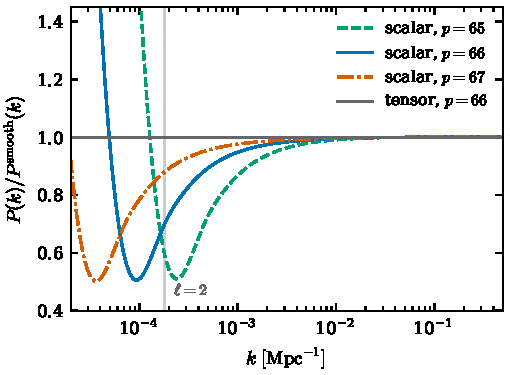
\includegraphics[width=\columnwidth]{figures/transfer}
\caption{Scalar power-spectrum transfer for the three viable invariant-wall
integers at the reheating-determined $N_*$, together with the tensor
transfer for $p=66$. The vertical line marks the quadrupole scale
$(\ell+\tfrac12)/\chi_*$ at $\ell=2$. A unit step in $p$ translates the
deficit by $e^{0.99}$ in $k$; the far-infrared rise at the left edge, which
exits the plotted range for $p=65$, is generated before classicalization and
lies outside the present horizon for all viable integers.}
\label{fig:transfer}
\end{figure}

Two computed negative results delimit the information carried by the feature.
First, the deficit is not generic to frozen-horizon exits: the
single-operator linear wall ($\alpha=0$, which has no fast-roll shoulder)
yields a maximal deficit of $1\%$, i.e.\ no observable feature. The
phenomenology requires $\alpha>0$ and hence both high-curvature operators;
reduced single-operator walls eliminate the signal. The intermediate
$d\ln R$ wall ($\alpha=2$, $S_{\max}=1.125$) produces a deficit of depth
$\simeq0.71$---the wall shape, and hence the depth, is independent of
$N_*$---so its low-$\ell$ signature is systematically weaker than either
branch analyzed here, and it is not carried through the likelihood pipeline.
Second, the integer $p$ is not
observable through the scalar two-point function beyond the feature's
location. A translation-invariant statistic---the rms difference of
$\ln P(k)$ between neighboring rungs after minimizing over a horizontal
shift and amplitude---measures $1.5\times10^{-3}$, falling to
$1.6\times10^{-4}$ once a tilt degenerate with the separately fitted
$(n_s,\alpha_s)$ is removed, against a numerical floor of $10^{-6}$
calibrated on same-$p$ pairs. A $0.02\%$ broadband shape difference
concentrated at cosmic-variance-limited multipoles is unmeasurable in
principle; consequently the data constrain only the joint combination of $p$
and the reheating completion, exactly as the degeneracy analysis of
Sec.~\ref{sec:reheating} implies.

\section{CMB projection and the official low-$\ell$ likelihood}
\label{sec:cmb}
The exact primordial tables are propagated through CAMB \cite{CAMB} with a
fixed Planck-2018 late-time cosmology; each featured spectrum is divided by
its own smooth continuation with the identical cosmology, so the radiation
transfer, reionization, lensing, and late integrated Sachs--Wolfe (ISW)
contributions cancel to first order in the ratio. CLASS \cite{CLASS}, fed the
same tables through an entirely separate input path, reproduces every ratio
at $\ell\le30$ to better than $6\times10^{-4}$. Table~\ref{tab:cmbratios}
shows the broad and narrow members of the invariant-wall branch, matching
the presentation of Table~\ref{tab:candidate} and Figs.~\ref{fig:transfer}
and~\ref{fig:clratios} (the branch's third viable integer, $p=67$, lies
closer still to the smooth limit); the coordinate branch exhibits the same
broad and narrow patterns one integer lower, and its likelihood values are
given in Table~\ref{tab:likelihood}.

Two properties of the transfer are relevant. The late ISW dilutes the temperature
signal---a Sachs--Wolfe-only estimate overstates the quadrupole suppression
by roughly a third---while $EE$, which carries no ISW, retains the deeper
imprint: for the broad pattern the $\ell=2$ ratios are $0.67$ in $EE$ against
$0.83$ in $TT$ (Table~\ref{tab:cmbratios}). This is the model-level counterpart of the long-standing
proposal to use large-angle polarization to test whether the low-$\ell$
deficit is primordial \cite{MortonsonHu2009,Cline2003,Billi2019}, with the
standard caveat that at these multipoles only the temperature-uncorrelated
component of $EE$ carries independent information. And the two surviving
rungs of each branch are distinguished
not by the quadrupole (both $\simeq18\%$ suppressed) but by the
\emph{width} of the suppression (Fig.~\ref{fig:clratios}): the broad pattern
reaches $C_3^{TT}/C_3^{\rm smooth}=0.73$ and persists past $\ell=10$, while
the narrow one is back above $0.92$ by $\ell=5$. This correlated $TT$--$TE$--$EE$ width
signature is the model family's only internal discriminant; both members
fall in the primordial low-$\ell$ suppression class that is the target of
forthcoming cosmic-variance-limited $E$-mode forecasts \cite{LiteBIRD2024}.
\begin{table*}[htbp]\centering
\begin{tabular}{r rrr rrr}
\hline
 & \multicolumn{3}{c}{$p=65$ (invariant, broad)} & \multicolumn{3}{c}{$p=66$ (invariant, narrow)} \\
$\ell$ & $TT$ & $EE$ & $TE$ & $TT$ & $EE$ & $TE$ \\
\hline
2 & 0.8372 & 0.6759 & 0.7384 & 0.8350 & 0.8139 & 0.7231 \\
3 & 0.7251 & 0.6728 & 0.5744 & 0.8757 & 0.8715 & 0.8120 \\
4 & 0.7480 & 0.7282 & 0.6335 & 0.9046 & 0.9008 & 0.8622 \\
5 & 0.7895 & 0.7713 & 0.7039 & 0.9238 & 0.9180 & 0.8926 \\
10 & 0.9038 & 0.9074 & 0.8764 & 0.9666 & 0.9683 & 0.9572 \\
20 & 0.9649 & 0.9518 & 0.9467 & 0.9881 & 0.9837 & 0.9820 \\
30 & 0.9824 & 0.9712 & 0.9666 & 0.9940 & 0.9902 & 0.9887 \\
\hline
\end{tabular}
\caption{Lensed $C_\ell$ ratios (featured over smooth) from CAMB at the reheating-determined $N_*$, for the two viable integers of the invariant-wall branch; the CAMB ratios are independently reproduced by CLASS to better than $6\times10^{-4}$ at every $\ell\le30$.}
\label{tab:cmbratios}
\end{table*}

\begin{figure*}
\centering
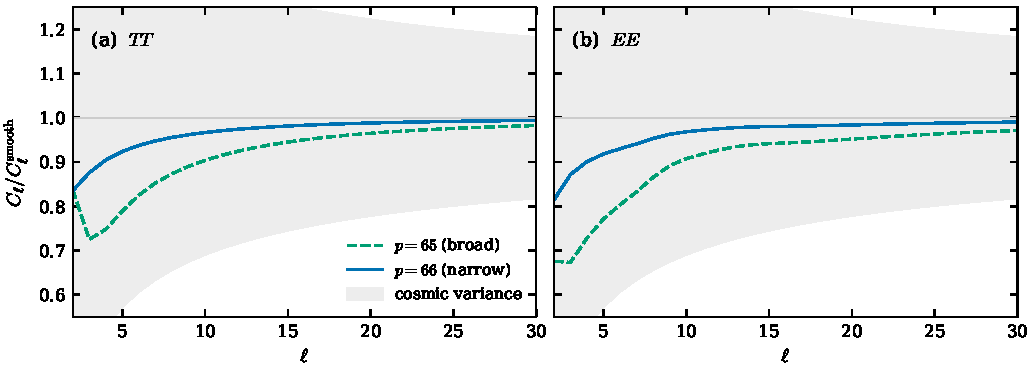
\includegraphics[width=0.92\textwidth]{figures/clratios}
\caption{Lensed $TT$ (a) and $EE$ (b) power ratios for the broad ($p=65$)
and narrow ($p=66$) invariant-wall integers; the shaded band shows the
per-multipole cosmic variance, which extends beyond the plotted range for
$\ell\lesssim4$. The two integers are distinguished by the
width of the suppression rather than by its depth at $\ell=2$. The entire
effect lies within cosmic variance, consistent with the marginalized
evidence of Table~\ref{tab:evidence}.}
\label{fig:clratios}
\end{figure*}

The confrontation with data uses the official Planck 2018 low-$\ell$
likelihoods \cite{Planck2018V}---the Gibbs/Blackwell--Rao Commander $TT$
likelihood and the SimAll probability-table $EE$ likelihood, in their exact
native implementations distributed with \textsc{cobaya} \cite{Cobaya},
validated on the Planck best-fit spectrum. Table~\ref{tab:likelihood} gives the result for
both branches at their reheating-determined $N_*$. A simpler diagnostic based
on diagonal errors for the released band powers overestimates the
polarization penalty of the broad pattern by an order of magnitude ($+1.7$,
against $+0.2$ from the exact non-Gaussian SimAll likelihood); all $EE$
contributions under the exact likelihood are below $0.7$ in magnitude, while
the temperature differences survive essentially unchanged.
\begin{table*}[htbp]\centering
\begin{tabular}{l r r r r}
\hline
Model & $\Delta\chi^2_{TT}$ & $\Delta\chi^2_{EE}$ & $\Delta\chi^2_{TT+EE}$ & \\
\hline
\multicolumn{5}{l}{\emph{coordinate wall ($\alpha=3$, $\xi_H=0$)}} \\
$p=62$ & +14.37 & -0.74 & +13.63 & excluded \\
$p=63$ & -0.16 & +0.23 & +0.07 &  \\
$p=64$ & -1.67 & -0.03 & -1.70 &  \\
$p=65$ & -0.70 & -0.01 & -0.71 &  \\
\hline
\multicolumn{5}{l}{\emph{invariant wall ($\alpha\simeq2.809$, $\xi_H=\tfrac16$)}} \\
$p=64$ & +9.10 & -0.63 & +8.47 & excluded \\
$p=65$ & -1.00 & +0.07 & -0.93 &  \\
$p=66$ & -1.55 & +0.00 & -1.55 &  \\
$p=67$ & -0.63 & +0.02 & -0.61 &  \\
\hline
\end{tabular}
\caption{Official Planck 2018 low-$\ell$ likelihoods (Commander $TT$, SimAll $EE$, exact native implementations): featured minus smooth, negative values favour the featured spectrum. Each model is compared against its own smooth continuation with identical late-time cosmology.}
\label{tab:likelihood}
\end{table*}


Three conclusions follow. First, the infrared rungs are excluded: the
members whose far-infrared rise enters the observable window fail at
$\Delta\chi^2=+13.4$ (coordinate branch, $p{=}62$) and $+8.5$ (invariant
branch, $p{=}64$). The integer ladder is therefore bounded from below in
both branches; this exclusion is the most stringent constraint obtained here. Second, the preferred rungs improve the fit by $-1.5$ to $-1.7$
--- of order one unit of $\chi^2$, obtained after the rung was located using
the same low multipoles, and therefore subject to a look-elsewhere penalty.
Third, marginalizing over the viable rungs with a flat prior, which is the
appropriate treatment of this selection freedom, yields an evidence of
$+0.9$ to $+1.1$, stable across branches and under pooling
(Table~\ref{tab:evidence}) and consistent with noise. The 2018 low-$\ell$
data thus exclude part of the model family and neither support nor disfavor
the remainder.
\begin{table}[htbp]\centering\small
\setlength{\tabcolsep}{4pt}
\begin{tabular}{l r}
\hline
Flat prior over & $2\ln(L_{\rm marg}/L_{\rm smooth})$ \\
\hline
coordinate wall, $p\in\{63,64,65\}$ & +0.93 \\
invariant wall, $p\in\{65,66,67\}$ & +1.08 \\
pooled, six viable integers & +1.01 \\
best single integer (no penalty) & +1.70 \\
\hline
\end{tabular}
\caption{Rung-marginalized evidence under the official low-$\ell$ likelihoods. Values of order unity are indistinguishable from noise; the difference from the best-single-integer row quantifies the look-elsewhere penalty.}
\label{tab:evidence}
\end{table}


The disposition of the full integer ladder follows from the monotonic trends
of Table~\ref{tab:likelihood}. Integers below the excluded member push the
deficit deeper into progressively better-measured multipoles and are
expected to be excluded a fortiori (not separately computed); integers above
the tested window move the deficit beyond the present horizon, rendering
those members observationally identical to Starobinsky inflation. Each
branch therefore consists of a hard lower edge, two to three live members,
and an infinite tail degenerate with the benchmark: the data select a finite
window of a discrete family; in this sense the construction is testable.

These numbers sit naturally in the published landscape. The Planck
exponential-cutoff extension improved the fit by $\Delta\chi^2\simeq-3.4$ at
the cost of two fitted parameters, with best-fit cutoff
$k_c\simeq3.4\times10^{-4}\Mpc$ \cite{Planck2015XX}; whipped-inflation
constructions reach $-10$ to $-13$ with two to four
\cite{Hazra2014,Hazra2016}; nested-sampling analyses of kinetic-dominance
cutoffs find the fit gain roughly cancelling the Occam penalty of a single
parameter \cite{Hergt2019a,Hergt2019b}; and a recent survey of
infrared-cutoff families reaches the same verdict \cite{Upadhyay2026}.
Against that economy of roughly three units of $\chi^2$ per fitted
parameter, $-1.5$ to $-1.7$ with no fitted feature parameter is competitive
--- the marginalized evidence of Table~\ref{tab:evidence} is the Bayesian
counterpart, with no Occam penalty to pay --- and it responds directly to
the a-posteriori-selection critique of low-multipole explanations
\cite{Bennett2011,Planck2018VII}. The complementary result is of greater consequence: because the members of the family carry no adjustable scale, they
can be rejected outright, and the $+13.4$ and $+8.2$ exclusions have no
analogue in continuous-cutoff fits, which the data can fail to reward but
can never exclude. We note finally that a suppression at
$k\simeq2$--$3\times10^{-4}\Mpc$ has been shown to move the large-angle
correlation statistic $S_{1/2}$ toward its observed low value
\cite{Melia2021,Copi2015}, so the surviving members inherit a second
large-angle consequence at no additional cost.

These results are confined to $\ell\le29$ at fixed late-time cosmology and
fixed $\tau$; the transfer-function cancellation in the ratio justifies this
for the feature itself, but the viable integers also differ slightly in
$n_s$, which enters the high-$\ell$ likelihood at an amplitude comparable to
the differences reported here. A joint $TT$, $TE$, $EE$ analysis with
late-time and nuisance parameters marginalized remains to be performed, and
the neutrality verdict is provisional until it is.

\section{Discussion}
\label{sec:discussion}
In summary, the inputs of the construction are: the observed scalar
amplitude; the integer $p$, whose integrality is derived from analyticity
while its value is empirical; the zero-work measure, for which invariance is
required but the choice among invariant measures remains free; the unit
spectral gap $\mu^2=d-1$, an independent axiom that cannot be derived within
the truncation; and the matter boundary condition $\xi_H$, for which the
conformal fixed-point value is symmetry-protected but not yet derived. The
causal-patch measure of the exit epoch, frequently listed among the
assumptions of such constructions, is demonstrably not an independent input
here: every observable is referenced to the end of inflation on a strongly
attracting trajectory, and no measurable quantity depends on where inflation
began.

The model determines the following observables with no remaining freedom:
$n_s\simeq0.962$--$0.964$, $r\simeq0.004$, a scalar deficit of depth
$\sim0.5$ at a computed wavenumber, no tensor counterpart above
$2\times10^{-3}$, no isocurvature, a squeezed bispectrum tracking the local
spectral slope through a sign change at the notch edges, and the correlated
$TT$--$TE$--$EE$ width pattern of Sec.~\ref{sec:cmb}. It is falsified by a
confirmed smooth scalar spectrum through the relevant low-$k$ window, by a
tensor notch correlated with the scalar one, by significant primordial
isocurvature, by a full-likelihood penalty exceeding the low-$\ell$ gain, or
by the failure of the ultraviolet program below. It has already lost one
member per branch to the Commander likelihood, and it cannot be confirmed by
the low-$\ell$ CMB at all: the deficit lies below cosmic variance, and a
feature lying below cosmic variance cannot be advanced as an explanation of
the low quadrupole.

The construction also carries a horizon-thermodynamic layer, which we record
because it bears on the open problem below. The Wald entropy
\cite{Wald1993} of the frozen horizon,
\begin{equation}
S_H=f_R(R_H)\,\frac{A_H}{4G}=\frac{96\pi^2 f_R(R_H)}{q}\frac{\Mpl^2}{M^2},
\end{equation}
obeys the exact identity $-I_E(S^4)=S_H$, extending the de Sitter relation
between Euclidean action and horizon entropy to this $f(R)$ saddle. Because the unit gap fixes
$f_R(R_H)=p(1+\alpha)/3$ while $q\simeq p(1+\alpha)$, the entropy reduces to
$32\pi^2(\Mpl/M)^2\,[1+\mathcal{O}(1/p)]\simeq1.8\times10^{12}$: it is set by
the observed scalar amplitude alone, to within a few percent across the
family, and lies some seventy-six orders of magnitude below the present
de~Sitter bound---a computably low-entropy initial condition. More
suggestively, the canonical measure of Sec.~\ref{sec:measure} is
$d\phi\propto d\ln f_R$, the logarithm of the Wald entropy coefficient, so
the zero-work condition states that the Einstein--Hilbert deficit integrates
to zero against the horizon-entropy coupling; and in the thermodynamic
derivation of the field equations, $f(R)$ gravity is precisely the case
requiring an internal entropy-production term generated by the variation of
$f_R$ \cite{Jacobson1995,EGJ2006,ChircoLiberati2010}. Whether the zero-work condition coincides
with that entropy balance is therefore a well-posed question. As established
in Appendix~\ref{app:entropy}, it does not, for two structural reasons: the $f(R)$ production term is a bulk viscosity, sign-definite in
the deviation, while the zero-work integrand is odd about the
Einstein--Hilbert baseline, so the second law itself forbids the
identification; and the apparent-horizon production of the Clausius
analysis \cite{AkbarCai2007} is, in vacuum, exactly $-dS_H$---a total
differential with no power to select $\alpha$. One element of the analysis is nevertheless
supportive: the reduced production functional is an integral
against $d\ln f_R$, so the thermodynamic framework independently singles
out the canonical measure of Sec.~\ref{sec:measure} as the natural one,
while leaving the zero-work condition itself underived.

The decisive open problem is ultraviolet, and it is well posed. Both
remaining arbitrary inputs are boundary data that a fixed-function equation
would supply: a regulator-independent $f(R)$ fixed function evaluated on the
inflationary trajectory would either satisfy a zero-work identity in some
definite measure---selecting $\alpha$---or not, and its analytic eigenoperator
spectrum would either contain the wall pair at some definite $p$---selecting
the rung---or not \cite{DietzMorris2012,BonannoContilloPercacci2010}. Either
outcome is decisive: a derivation would convert the feature location into a
parameter-free prediction testable through the width pattern, while a
refutation would falsify the construction independently of any data. Until
then, the model is a nonsingular completion of the observational benchmark
that is indistinguishable from it at high multipoles, partially excluded at
low multipoles, and otherwise consistent with current data at the level of
$+1.0$ units of marginalized evidence.

\section{Conclusions}
\label{sec:conclusions}
The principal results of this work are the following.

\begin{enumerate}
\item Two additional curvature operators, $R^{\,p+1}$ and $R^{\,2p+1}$, give
metric $f(R)$ gravity an exact constant-curvature solution at $R_H=qM^2$
carrying a single unstable scalaron direction. Starobinsky's original
nonsingular scenario---birth in an unstable de Sitter state that decays into
scalaron-driven inflation---is thereby realized within a local, polynomial,
metric theory, with the horizon curvature and the instability rate as
independent algebraic data rather than as outputs of the conformal anomaly.

\item The integrality of $p$ follows from analyticity of the action at
$R=0$, so the family of completions is discrete rather than continuous. Two
inputs remain free: the value of $p$, and the integration measure entering
the zero-work condition.

\item The wavenumber of the primordial feature is exactly degenerate with
the reheating history, and no fit can break the degeneracy. Because the
low-curvature limit is exactly Starobinsky, the reheating history is
computable: solving the coupled scalaron--radiation system gives
$N_*=50.6$--$51.6$ with an uncertainty of $0.2$ e-folds against an integer
spacing of $0.94$--$0.99$, so that each integer predicts a definite feature
location. The results indicate that feature models generally require a
computed reheating history before a feature scale can be claimed.

\item The predicted spectra exhibit a scalar deficit of depth $\simeq0.5$
with no tensor counterpart above $2\times10^{-3}$. Two negative results
delimit the information the feature carries: the deficit requires both
high-curvature operators, the single-operator wall producing a $1\%$ effect;
and $p$ is not observable through the scalar two-point function beyond the
feature location.

\item Under the official Planck 2018 low-$\ell$ likelihoods, one integer of
each branch is excluded ($\Delta\chi^2=+13.4$ and $+8.5$), while the
preferred integers give $\Delta\chi^2_{TT+EE}=-1.5$ to $-1.7$. Marginalized
over the integer ladder the evidence is $+1.0$, consistent with a
statistical fluctuation. The findings therefore constrain the family from
below while neither supporting nor disfavouring the remainder, and the
deficit itself lies below cosmic variance.

\item The Wald entropy of the frozen horizon satisfies $-I_E(S^4)=S_H$ and
reduces to $\simeq1.8\times10^{12}$, fixed by the observed scalar amplitude.
The zero-work condition is not an entropy balance, for reasons given in
Appendix~\ref{app:entropy}, although the thermodynamic analysis
independently selects the canonical measure.
\end{enumerate}

Two calculations would materially change these conclusions: a joint
$TT$, $TE$, $EE$ likelihood with late-time and nuisance parameters
marginalized, which would render the present neutrality verdict definitive
or overturn it; and a regulator-independent fixed-function analysis, which
would either supply the zero-work measure and the realized integer or
falsify the construction independently of any data.

\section*{Declarations}
\paragraph{Funding.} No funding was received for this work.
\paragraph{Conflict of interest.} The author declares no competing
interests.
\paragraph{Use of AI tools.} The author used Anthropic's Claude to assist
with the code, figures, and text; the author verified all results and takes
full responsibility for the content.
\paragraph{Data and code availability.} All numerical results in this paper
regenerate from the released code, archived at
\href{https://doi.org/10.5281/zenodo.21829379}{doi:10.5281/zenodo.21829379}
and developed at \url{https://github.com/spsingularity/frozen-horizon},
which contains the full pipeline from the action to the
likelihood evaluation; every table and figure in this manuscript is a build
artifact of that pipeline.

\appendix

\section{The unit gap cannot be derived within the truncation}
\label{app:unitgap}
The one-loop scalar contribution of the four-sphere saddle is formally
\begin{align}
\Gamma_1(\mu^2)&=\frac12\sum_{L=0}^{\infty}d_L
\ln\left|L(L+3)-\mu^2\right|,\nonumber\\
d_L&=\frac{(L+1)(L+2)(2L+3)}{6}.
\end{align}
Any attempt to select $\mu^2$ by extremizing this determinant requires
\begin{equation}
\frac{\partial\Gamma_1}{\partial\mu^2}
=-\frac12\sum_{L=0}^{\infty}\frac{d_L}{L(L+3)-\mu^2},
\end{equation}
whose summand grows linearly at large $L$: the derivative is ultraviolet
divergent, and the counterterms that absorb the divergence carry finite
renormalized parts that displace any stationary point. Consequently neither
$\mu^2=3$ nor any other value can be derived from the one-loop determinant
of the finite $f(R)$ truncation in a regulator-independent way. The unit gap
can become a prediction only within a UV-complete effective action with a
specified renormalization condition, or from a symmetry fixing the
four-sphere fluctuation operator; within the present theory it is an
irreducible axiom, and it is reported as such in Sec.~\ref{sec:discussion}.

\section{The zero-work condition is not an entropy balance}
\label{app:entropy}
Three facts establish the negative result quoted in
Sec.~\ref{sec:discussion}.

\emph{(i) The apparent-horizon production is a state function.} For vacuum
spatially flat FRW in $f(R)$ gravity, the Clausius analysis of the apparent
horizon assigns an internal production
$d\bar S=-(A/4GH)\,\ddot F\,dt$ with $F\equiv f_R$ \cite{AkbarCai2007}.
Differentiating the Wald entropy $S_{\rm W}=FA/4G$ with $A=4\pi/H^2$ and
using the vacuum field equation $2F\dot H=H\dot F-\ddot F$ gives
$\dot S_{\rm W}=(A/4GH)(H\dot F-2F\dot H)=(A/4GH)\,\ddot F$, hence
\begin{equation}
d\bar S=-\,dS_{\rm W}
\end{equation}
exactly: the accumulated production across the wall is endpoint data and
cannot select the wall coefficient. (A corollary follows: the Wald
entropy \emph{decreases} monotonically across the wall, $F$ falling faster
than the horizon area grows---a distinctive signature of the frozen-horizon
exit.)

\emph{(ii) The local production is sign-definite.} In the
Eling--Guedens--Jacobson framework the $f(R)$ production term is a bulk
viscosity, $\sigma\propto F\,\tilde\theta^{\,2}$ with
$\zeta=3F/16\pi G$ \cite{EGJ2006,ChircoLiberati2010}: positive definite in
the deviation. The zero-work integrand $(S-1)$ is odd about the
Einstein--Hilbert baseline $S=1$. A sign-definite functional cannot
reproduce an odd condition, and the second law forbids its vanishing for
any $\alpha$; numerically, for $p=63$ and $p=66$, the accumulated wall
production is positive and monotone increasing in $\alpha$ throughout
$1\le\alpha\le6$, with no interior extremum, so neither a vanishing nor a
minimal-production reading selects a wall.

\emph{(iii) The measure emerges anyway.} In slow roll through the wall the
accumulated production reduces to
\begin{equation}
\Sigma\;\propto\;\int_0^1 S(z)\,\frac{J}{4J-1}\;d\ln f_R,
\qquad J\equiv\frac{Rf_{RR}}{f_R},
\end{equation}
an integral against $d\ln f_R$: the thermodynamic framework independently
selects the canonical entropy-coupling measure adopted in
Sec.~\ref{sec:measure}, with weight $S$ (the heat-flow rate) rather than
$S-1$. The zero-work condition is therefore properly read as stationarity
of the integrated Einstein--Hilbert deficit in that measure, not as an
entropy balance, and its derivation remains open.

\bibliographystyle{spphys}
\bibliography{refs}

\end{document}
